\chapter{ Chapitre 7 : Sprint 4 "Gestion \centering des Publications   et des Notifications"}
\begin{spacing}{1.2}
\minitoc
\thispagestyle{MyStyle}
\end{spacing}
\newpage
\begin{sloppypar} 

\section{Introduction }
\vspace{-4mm}
Dans ce sprint, nous nous concentrons sur l'amélioration de nos publications et notifications pour une expérience utilisateur plus engageante. Nous travaillerons sur l'optimisation de l'interface de publication, l'ajout de fonctionnalités de réaction, ainsi que sur l'amélioration de la gestion des notifications pour une distribution plus ciblée. 

\vspace{-1cm}
\section{Backlog du sprint}
\vspace{-4mm}
Le backlog de gestion des publications et des notifications comprend des tâches telles que la création, la modification et la suppression de publications, ainsi que la gestion des notifications automatiques et personnalisées. Cela permettra de garantir une diffusion efficace de l'information et une interaction fluide entre les utilisateurs et l'application.
\vspace{-1mm}
\begin{table}[h]
\centering
\begin{tabular}{|p{8cm}|p{3cm}|p{3cm}|}
\hline
\textbf{ Tâches } & \textbf{ Priorité }& \textbf{Période/jour}  \\
\hline En tant qu’un étudiant ,je peux consulter les publications de ma page d’accueil dans l’application mobile.& Élevée  & 5 jours \\
\hline En tant qu’un étudiant ,je peux consulter mes publications de ma page profile dans l’application mobile.  & Élevée  & 4 jours  \\
\hline En tant qu’un étudiant ,je peux commenter et réagir aux publications dans l’application mobile.  & Élevée  & 7 jours  \\
\hline En tant qu’un étudiant ,je peux supprimer mes publications dans l’application mobile.  & Élevée  & 7 jours  \\
\hline En tant qu'un utilisateur, je peux créer  des notifications personnalisés  sur la partie web  & Élevée  & 7 jours  \\
\hline En tant qu’un étudiant ,je peux commenter et réagir aux publications dans l’application mobile.  & Élevée  & 7 jours  \\
\hline

\end{tabular}
\caption{Tableau de Backlog de produit Sprint 4}
\end{table}
\vspace{-1.2cm}

\section{L'Algorithme des publications}
\vspace{-4mm}
L'algorithme de publication de notre application mobile est conçu pour équilibrer la visibilité entre les nouvelles publications et les publications populaires. Lors de la création de chaque publication, celle-ci commence avec une priorité de 100 points. Pour chaque "j'aime" reçu, la publication gagne 0,1 point, tandis que chaque commentaire lui apporte 0,3 point. Cependant, pour maintenir un flux dynamique et pertinent de contenu, chaque publication perd 1 point de priorité chaque heure. L'algorithme s'assure que les utilisateurs voient les contenus les plus pertinents et intéressants en affichant en priorité les 10 publications les plus récentes ainsi que les 10 publications ayant accumulé le plus de points. Cette approche garantit une visibilité équilibrée entre les nouvelles publications et celles qui suscitent le plus d'engagement.
\vspace{-1cm}
\section{Les Notifications }
\vspace{-4mm}
Notre application mobile intègre un système de notifications pour garantir que les utilisateurs restent informés des activités et des mises à jour importantes. Il existe deux types de notifications : les notifications automatiques générées par le système et les notifications personnalisées créées par l'administrateur.

Les notifications automatiques sont déclenchées lorsque l'administrateur ajoute un nouvel événement ou un nouveau stage. Ces notifications assurent que tous les utilisateurs concernés reçoivent rapidement l'information pertinente sans intervention manuelle supplémentaire de l'administrateur.

En outre, l'administrateur a la possibilité de créer des notifications personnalisées pour des cas spécifiques. Cela permet de communiquer des messages ciblés et spécifiques aux utilisateurs selon les besoins particuliers. Ces notifications personnalisées peuvent être utilisées pour des annonces importantes, assurant ainsi une flexibilité et une réactivité accrues dans la gestion des informations.

\vspace{-1cm}

\section {Analyse et spécification des besoins}
\vspace{-4mm}
Afin de mieux comprendre la structure de notre système, nous avons utilisé un diagramme de cas d'utilisations qui est présenté ci-dessous.
\vspace{-4mm}
\subsection{Diagramme de cas d’utilisation détaillé}
\vspace{-4mm}
Le diagramme de cas d'utilisation pour les notifications et les publications décrit les interactions entre les utilisateurs et le système pour créer, gérer et consulter des notifications et des publications.
\vspace{-4mm}
\begin{figure}[H]%
    \center%
    \setlength{\fboxsep}{5pt}%
    \setlength{\fboxrule}{0.5pt}%
    \fbox{
    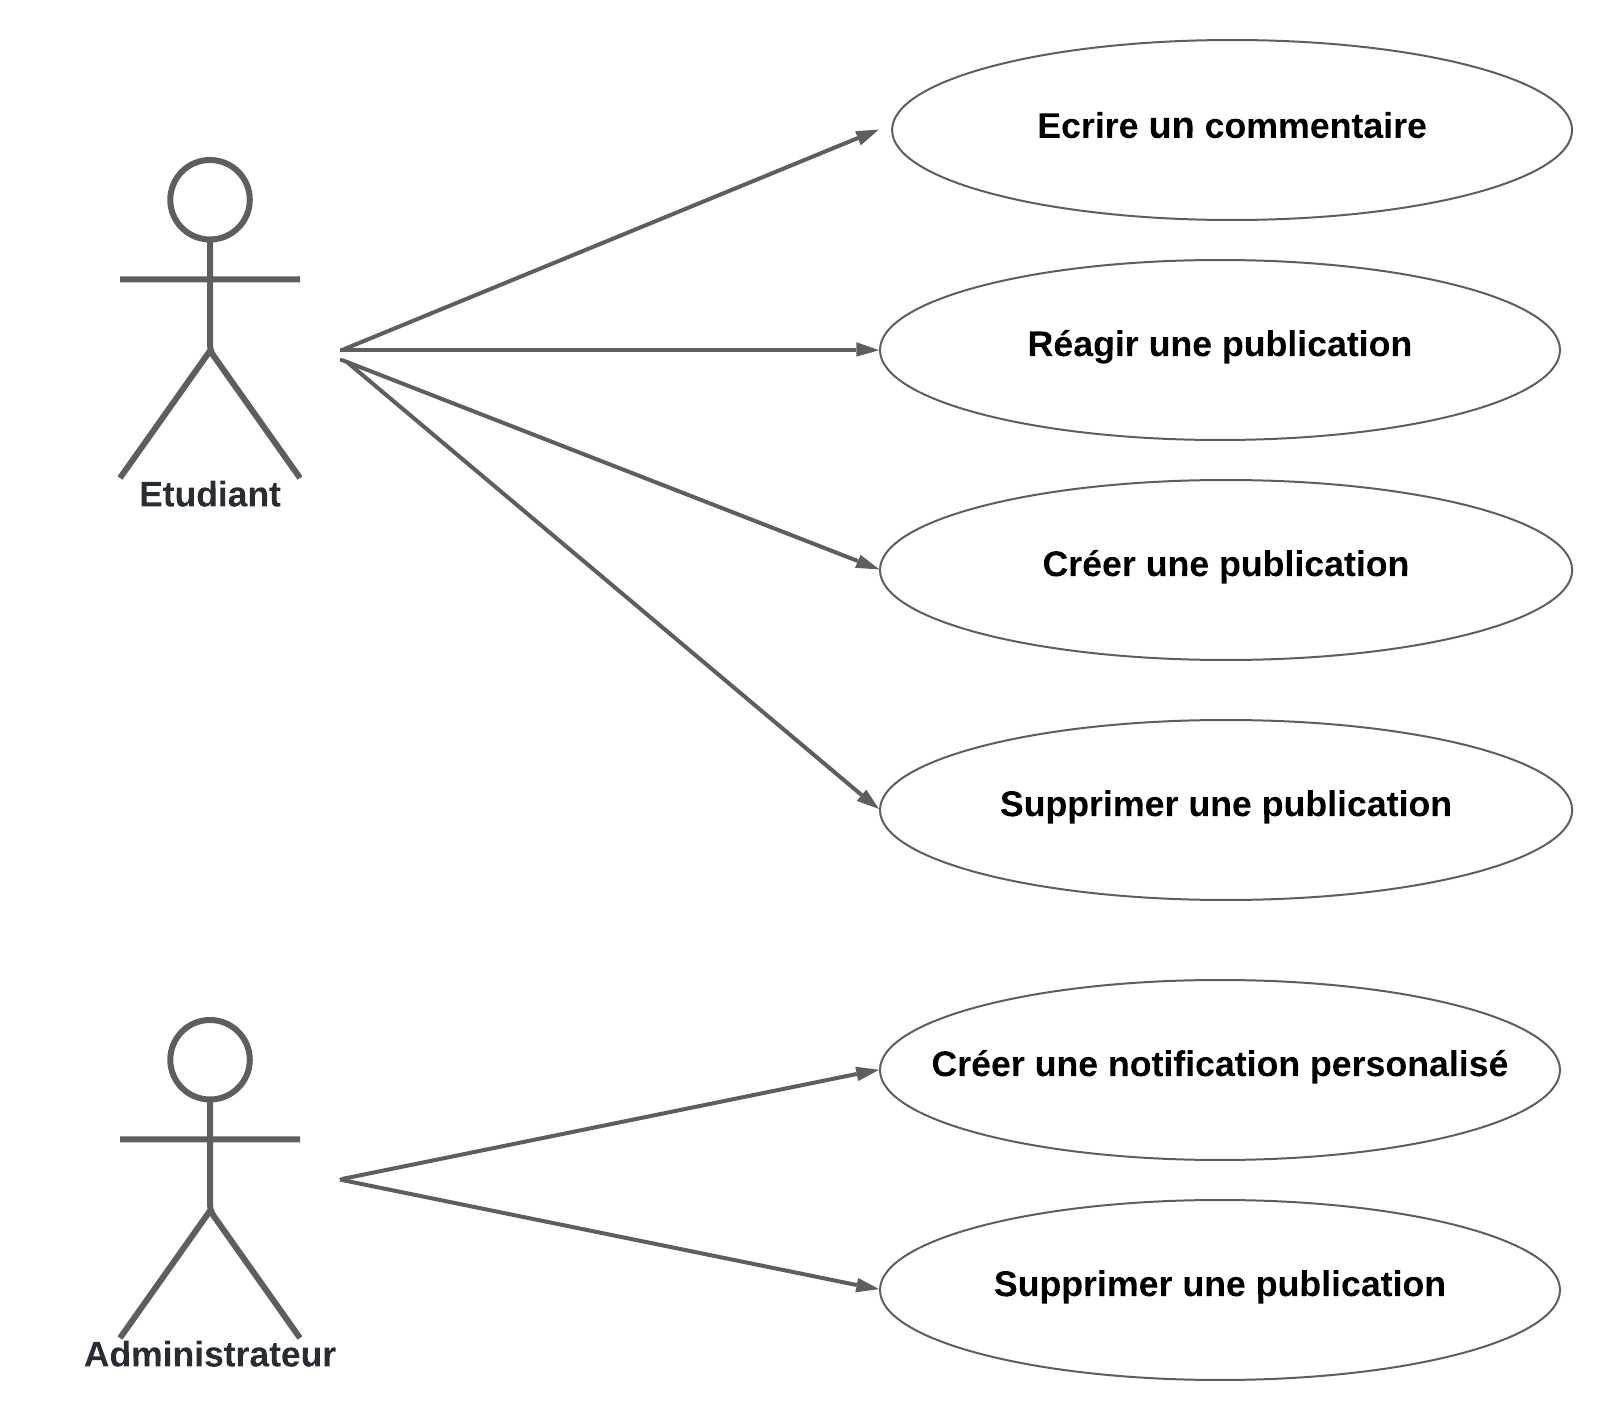
\includegraphics[height=10cm,width=13cm]{images/AAADiagramDesCasPubsNotifs.png}%
    }
    \caption{Diagramme de cas d'utilisation Sprint 4 }
\end{figure}

\vspace{-6mm}
Voici la description mise à jour du cas d'utilisation "Créer une publication" :
\vspace{-9mm}
\subsection{Description textuelle du cas d’utilisation « Créer une publication »}
\vspace{-4mm}
Le tableau ci-dessous détaille le cas d'utilisation "Créer une publication" dans le cadre d'un système où les utilisateurs peuvent publier du contenu après s'être authentifiés.

\begin{table}[h]
\centering
\begin{tabular}{|p{3cm}|p{11cm}|}
\hline
\textbf{Cas d'utilisation } & Créer une publication \\
\hline
\textbf{Acteurs} & Utilisateur \\
\hline
\textbf{Précondition} & Utilisateur authentifié \\
\hline
\textbf{Postcondition} & Publication créée \\
\hline
\textbf{Scénario nominal} & 
\begin{enumerate}
    \item L'utilisateur est sur la page d'accueil.
    \item L'utilisateur clique sur le bouton « Créer une publication ».
    \item Le système affiche le formulaire de création de publication.
    \item L'utilisateur rédige sa publication.
    \item L'utilisateur clique sur le bouton "Publier".
\end{enumerate} \\
\hline
\textbf{Exception} & 
Un champ au moins doit être rempli dans le formulaire de création de publication. Le système affiche un message d'erreur si aucun champ n'est rempli. \\
\hline
\end{tabular}
\caption{Description du cas d’utilisation « Créer une publication »}
\end{table}
\vspace{-4mm}
Voici la description mise à jour du cas d'utilisation "Créer une notification personnalisée" :
\vspace{-1cm}
\subsection{Description textuelle du cas d’utilisation « Créer une notification personnalisée »}
\vspace{-4mm}
Le tableau ci-dessous détaille le cas d'utilisation "Créer une notification personnalisée" dans le cadre d'un système où les administrateurs peuvent envoyer des notifications personnalisées après s'être authentifiés.

\begin{table}[h]
\centering
\begin{tabular}{|p{3cm}|p{11cm}|}
\hline
\textbf{Cas d'utilisation } & Créer une notification personnalisée \\
\hline
\textbf{Acteurs} & Administrateur \\
\hline
\textbf{Précondition} & Administrateur authentifié \\
\hline
\textbf{Postcondition} & Notification créée et envoyée \\
\hline
\textbf{Scénario nominal} & 
\begin{enumerate}
    \item L'administrateur est sur la page d'accueil du dashboard.
    \item L'administrateur navigue dans le sidebar et clique sur le bouton "Notifications".
    \item Le système affiche le formulaire de création de notification.
    \item L'administrateur remplit les champs nécessaires de la notification.
    \item L'administrateur clique sur le bouton "Envoyer".
\end{enumerate} \\
\hline
\textbf{Exception} & 
Tous les champs du formulaire de création de notification doivent être remplis. Le système affiche un message d'erreur si un champ est laissé vide. \\
\hline
\end{tabular}
\caption{Description du cas d’utilisation « Créer une notification personnalisée »}
\end{table}
\vspace{-1cm}
\section{Diagramme de séquence }
\vspace{-4mm}
Pour mieux visualiser les interactions entre l'utilisateur et le système lors de la création de publications et de notifications, nous avons utilisé des diagrammes de séquence. Ces diagrammes décrivent de manière détaillée les étapes impliquées dans la création de publications par les utilisateurs ainsi que la génération de notifications par l'administrateur.
\vspace{-1.5cm}
\subsection{Diagramme de séquence «Créer une publication»}
\vspace{-4mm}
Le diagramme de séquence "Créer une publication" illustre le flux d'actions entre l'utilisateur et le système lorsqu'il souhaite publier du contenu sur l'application. Ce diagramme détaille les étapes telles que l'ouverture de la page de création de publication, la saisie du contenu, et la publication effective de la publication.
\vspace{-4mm}
\begin{figure}[H]%
    \center%
    \setlength{\fboxsep}{5pt}%
    \setlength{\fboxrule}{0.5pt}%
    \fbox{
    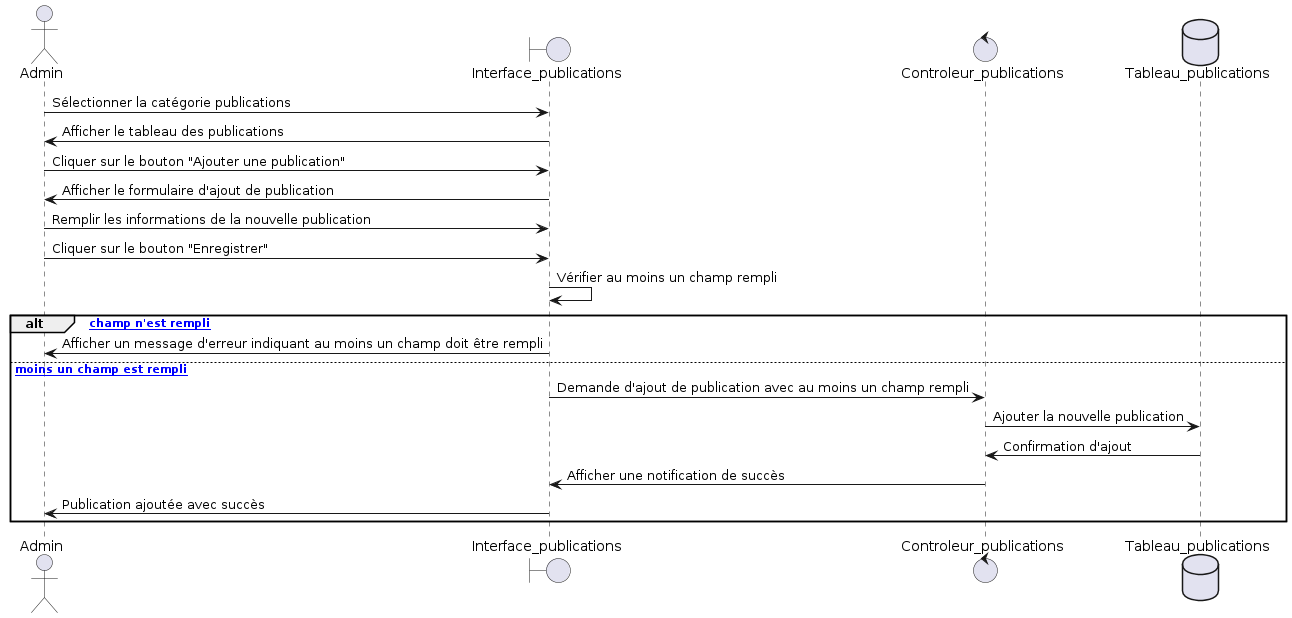
\includegraphics[height=9cm,width=15cm]{images/ffffpublications.png}%
    }
    \caption{Diagramme de séquence créer une publication }
\end{figure}
\vspace{-18mm}
\subsection{Diagramme de séquence «Créer une notification»}
\vspace{-4mm}
Le diagramme de séquence "Créer une notification" montre comment un administrateur crée une notification personnalisée dans le système, ce qui déclenche l'envoi de la notification aux utilisateurs concernés.

\begin{figure}[H]%
    \center%
    \setlength{\fboxsep}{5pt}%
    \setlength{\fboxrule}{0.5pt}%
    \fbox{
    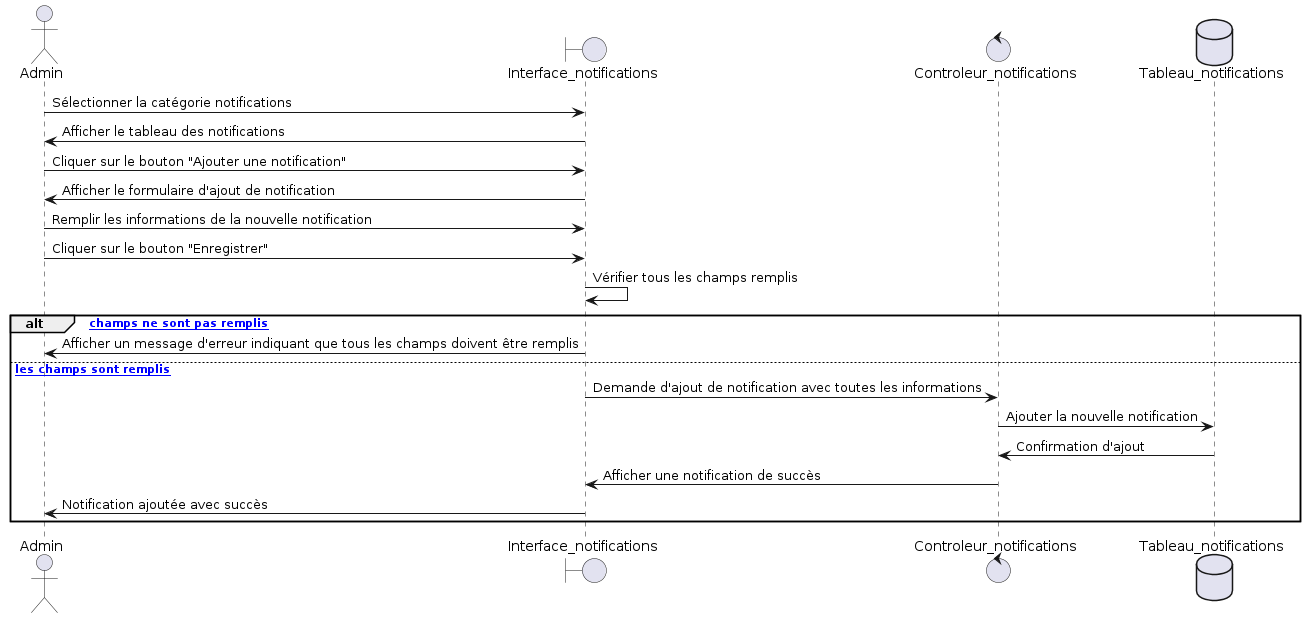
\includegraphics[height=9cm,width=15cm]{images/fffffnotification.png}%
    }
    \caption{Diagramme de séquence «Créer une notification» }
\end{figure}


\section{Diagramme de classes detaillé }
\vspace{-4mm}
Le diagramme de classes présenté ci-dessus illustre la gestion des publications et des notifications dans notre système. 

\begin{figure}[H]%
    \center%
    \setlength{\fboxsep}{5pt}%
    \setlength{\fboxrule}{0.5pt}%
    \fbox{
    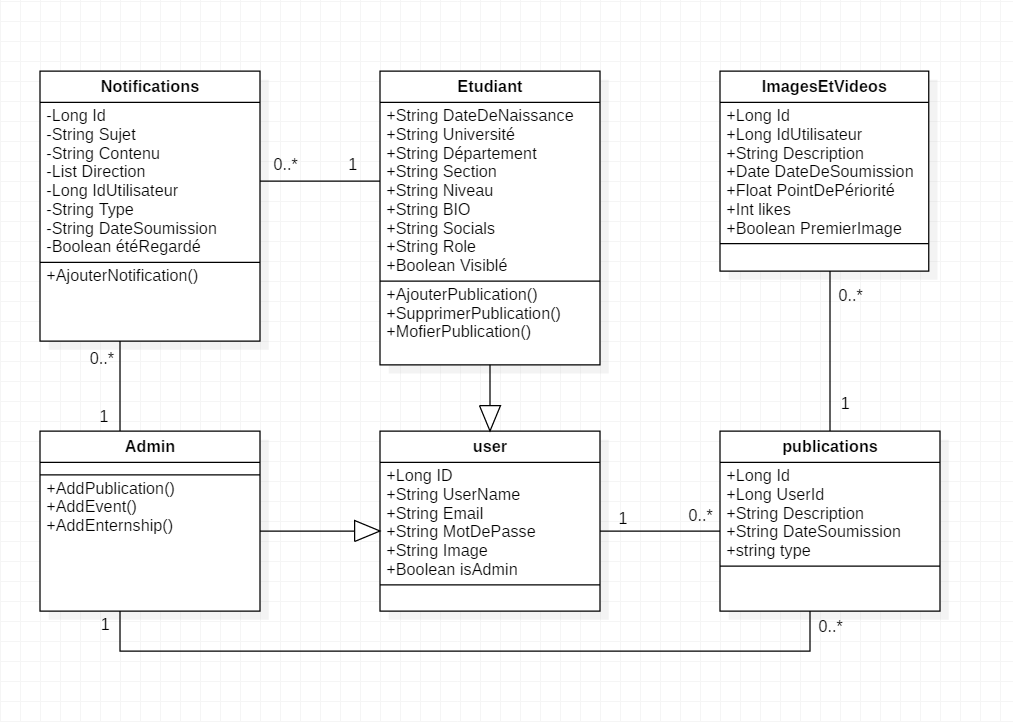
\includegraphics[height=15cm,width=15cm]{images/AAANotificatiosnPubs.png}%
    }
    \caption{Diagramme de classes Sprint 4}
\end{figure}
\vspace{-1cm}

\section{Réalisation }
\vspace{-6mm}
\subsection{Page créer une publication}
\vspace{-4mm}
La page "Créer une publication" dans la partie mobile permet à l'utilisateur de rédiger et de publier du contenu.
\vspace{-4mm}
\begin{figure}[H]%
    \center%
    \setlength{\fboxsep}{5pt}%
    \setlength{\fboxrule}{0.5pt}%
    \fbox{
    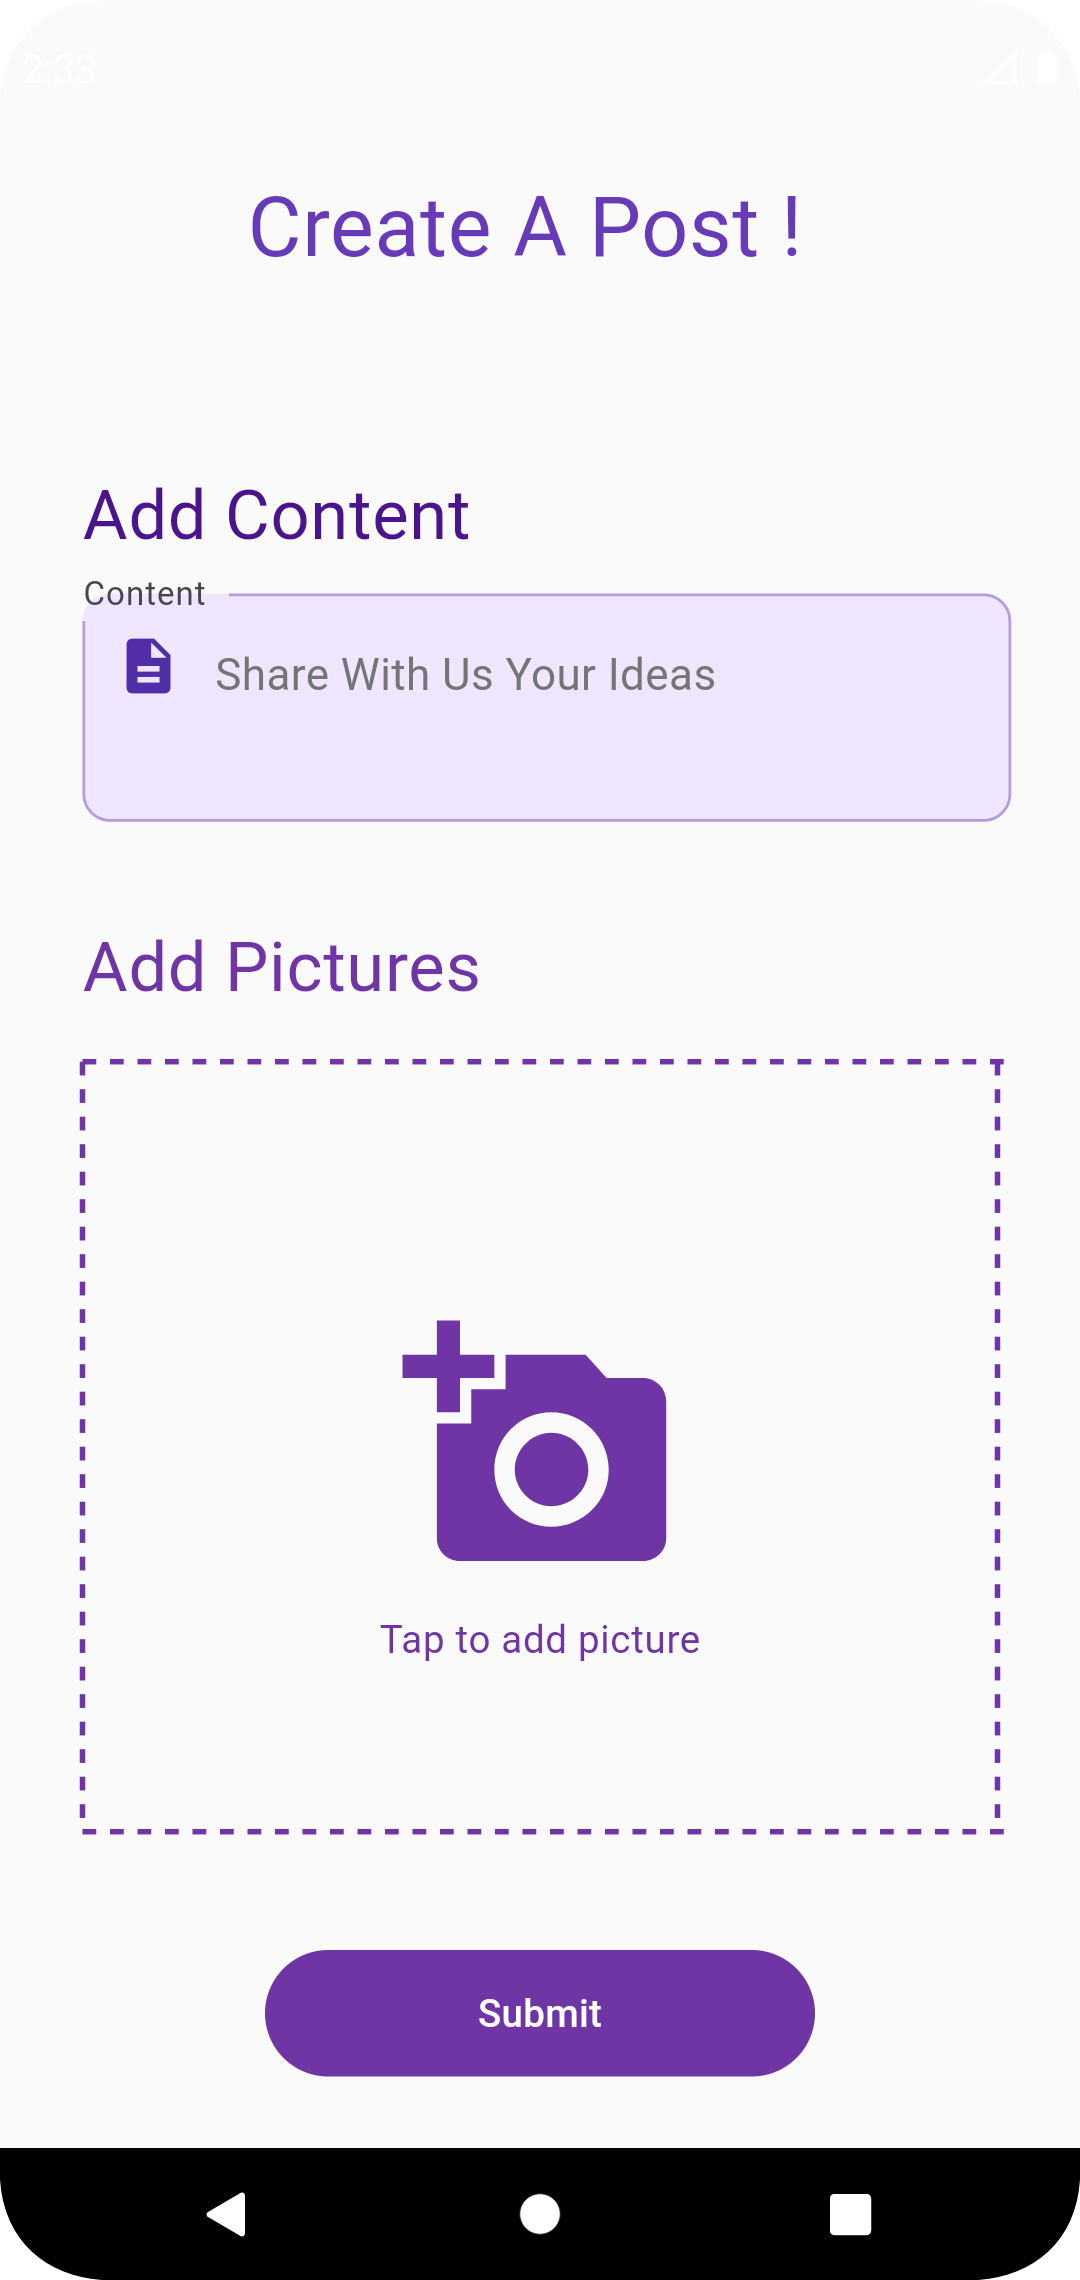
\includegraphics[height=9.8cm,width=7cm]{images/AddPostPage.png}%
    }
    \caption{Interface créer une publication}
\end{figure}
\vspace{-1.8cm}
\section{Interface commenter et réagir sur une publication}
\vspace{-8mm}
Les utilisateurs peuvent commenter ou réagir aux publications avant même de consulter les commentaires et réactions des autres utilisateurs.
\begin{figure}[H]%
    \center%
    \setlength{\fboxsep}{5pt}%
    \setlength{\fboxrule}{0.5pt}%
    \fbox{
    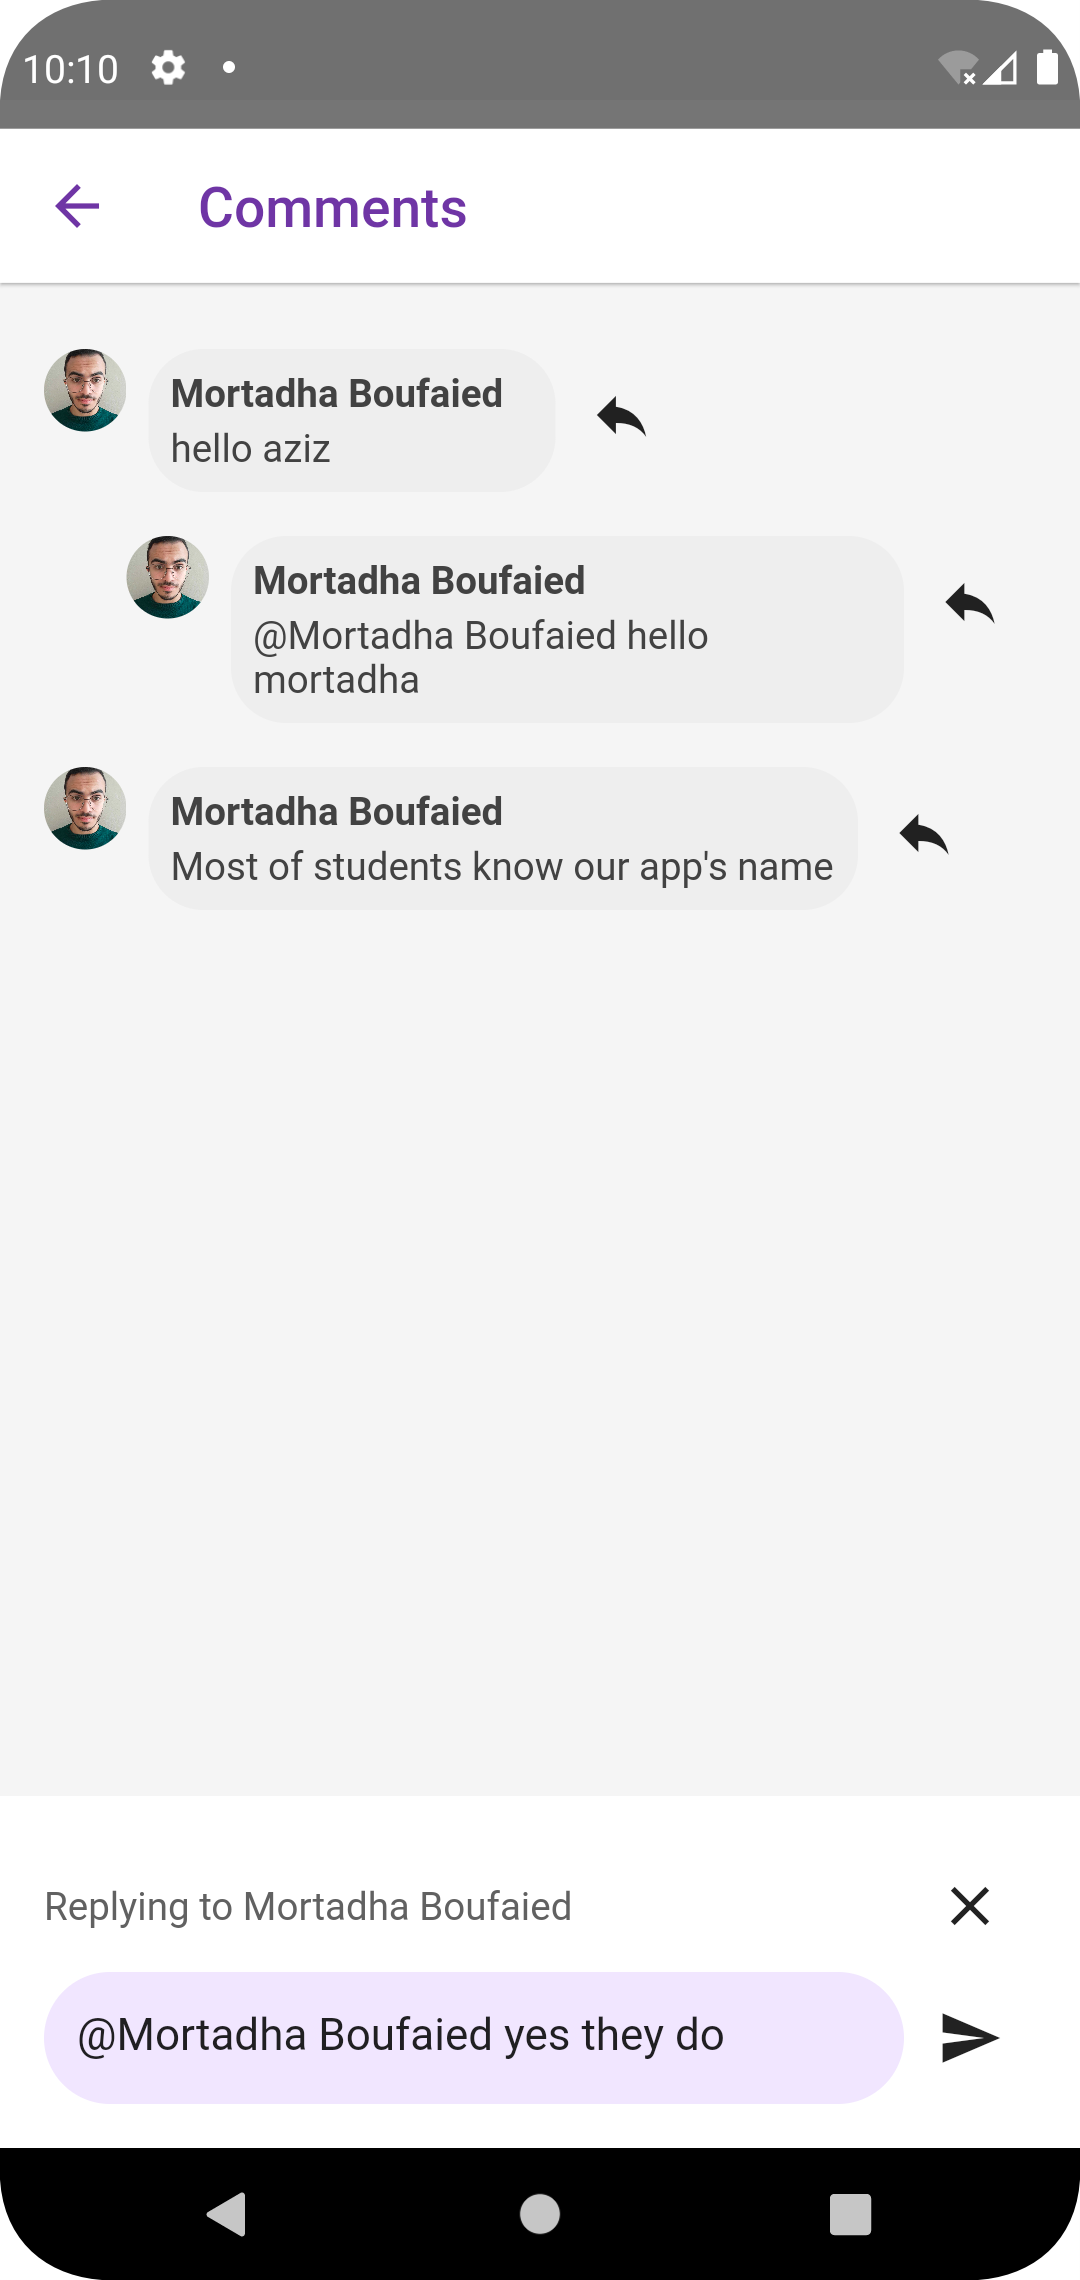
\includegraphics[height=9.8cm,width=7cm]{images/XCommentsBar.png}%
    }
    \caption{Interface ajout d'un commentaire }
\end{figure}

\vspace{-10mm}
\subsection{Interface Acceuil mobile }
\vspace{-7mm}
Sur la page d'accueil de l'application mobile, toutes les publications sont visibles.
\vspace{-2mm}
\begin{figure}[H]%
    \center%
    \setlength{\fboxsep}{5pt}%
    \setlength{\fboxrule}{0.5pt}%
    \fbox{
    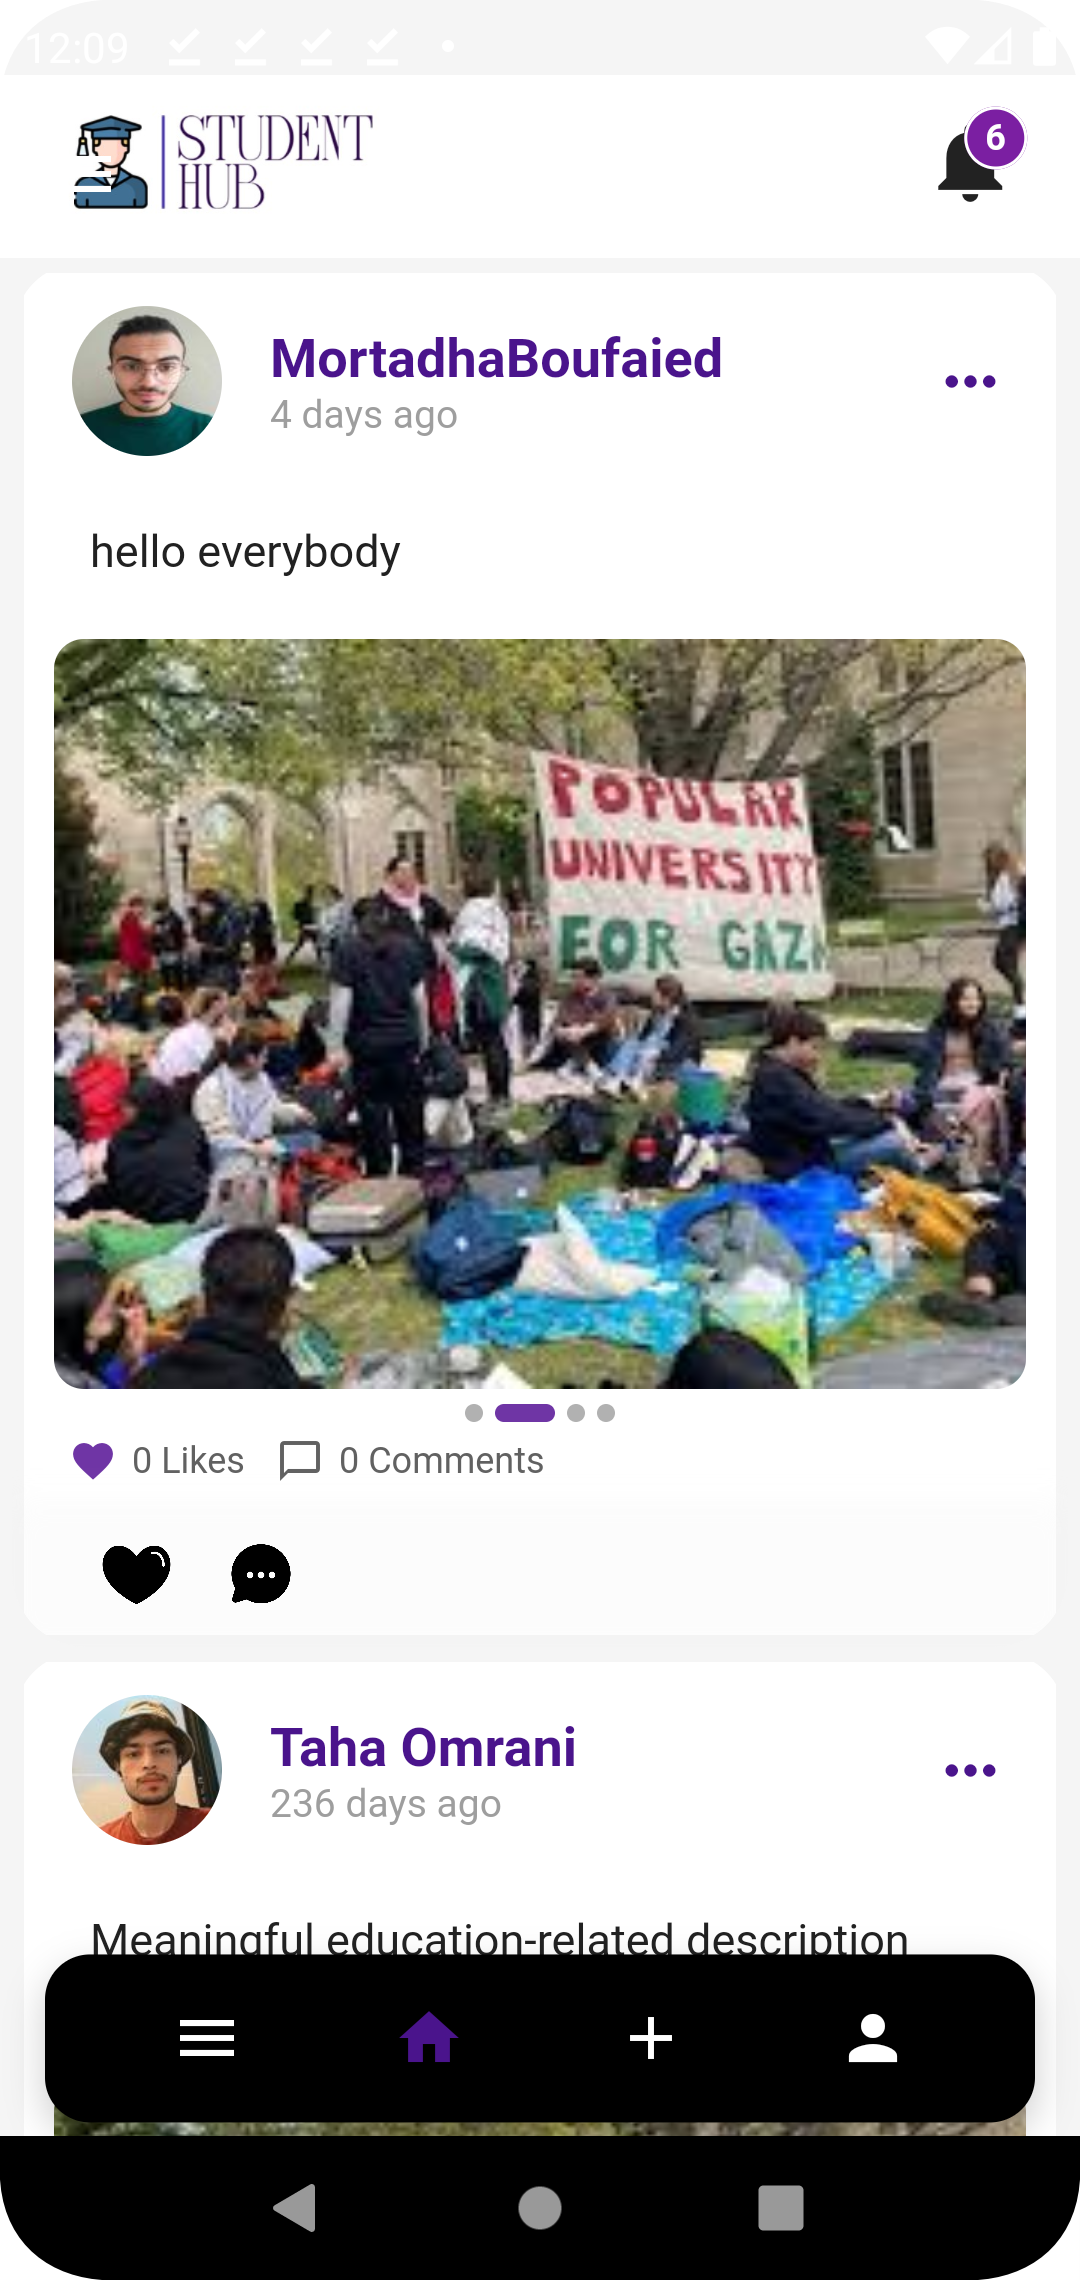
\includegraphics[height=9.5cm,width=7cm]{images/AAAHomePage.png}%
    }
    \caption{Interface page d'accueil partie mobile}
\end{figure}

\vspace{-1.8cm}
\subsection{Interface Notification mobile }
\vspace{-7mm}
La page de notifications affiche les notifications reçues par l'utilisateur.
\vspace{-2mm}
\begin{figure}[H]%
    \center%
    \setlength{\fboxsep}{5pt}%
    \setlength{\fboxrule}{0.5pt}%
    \fbox{
    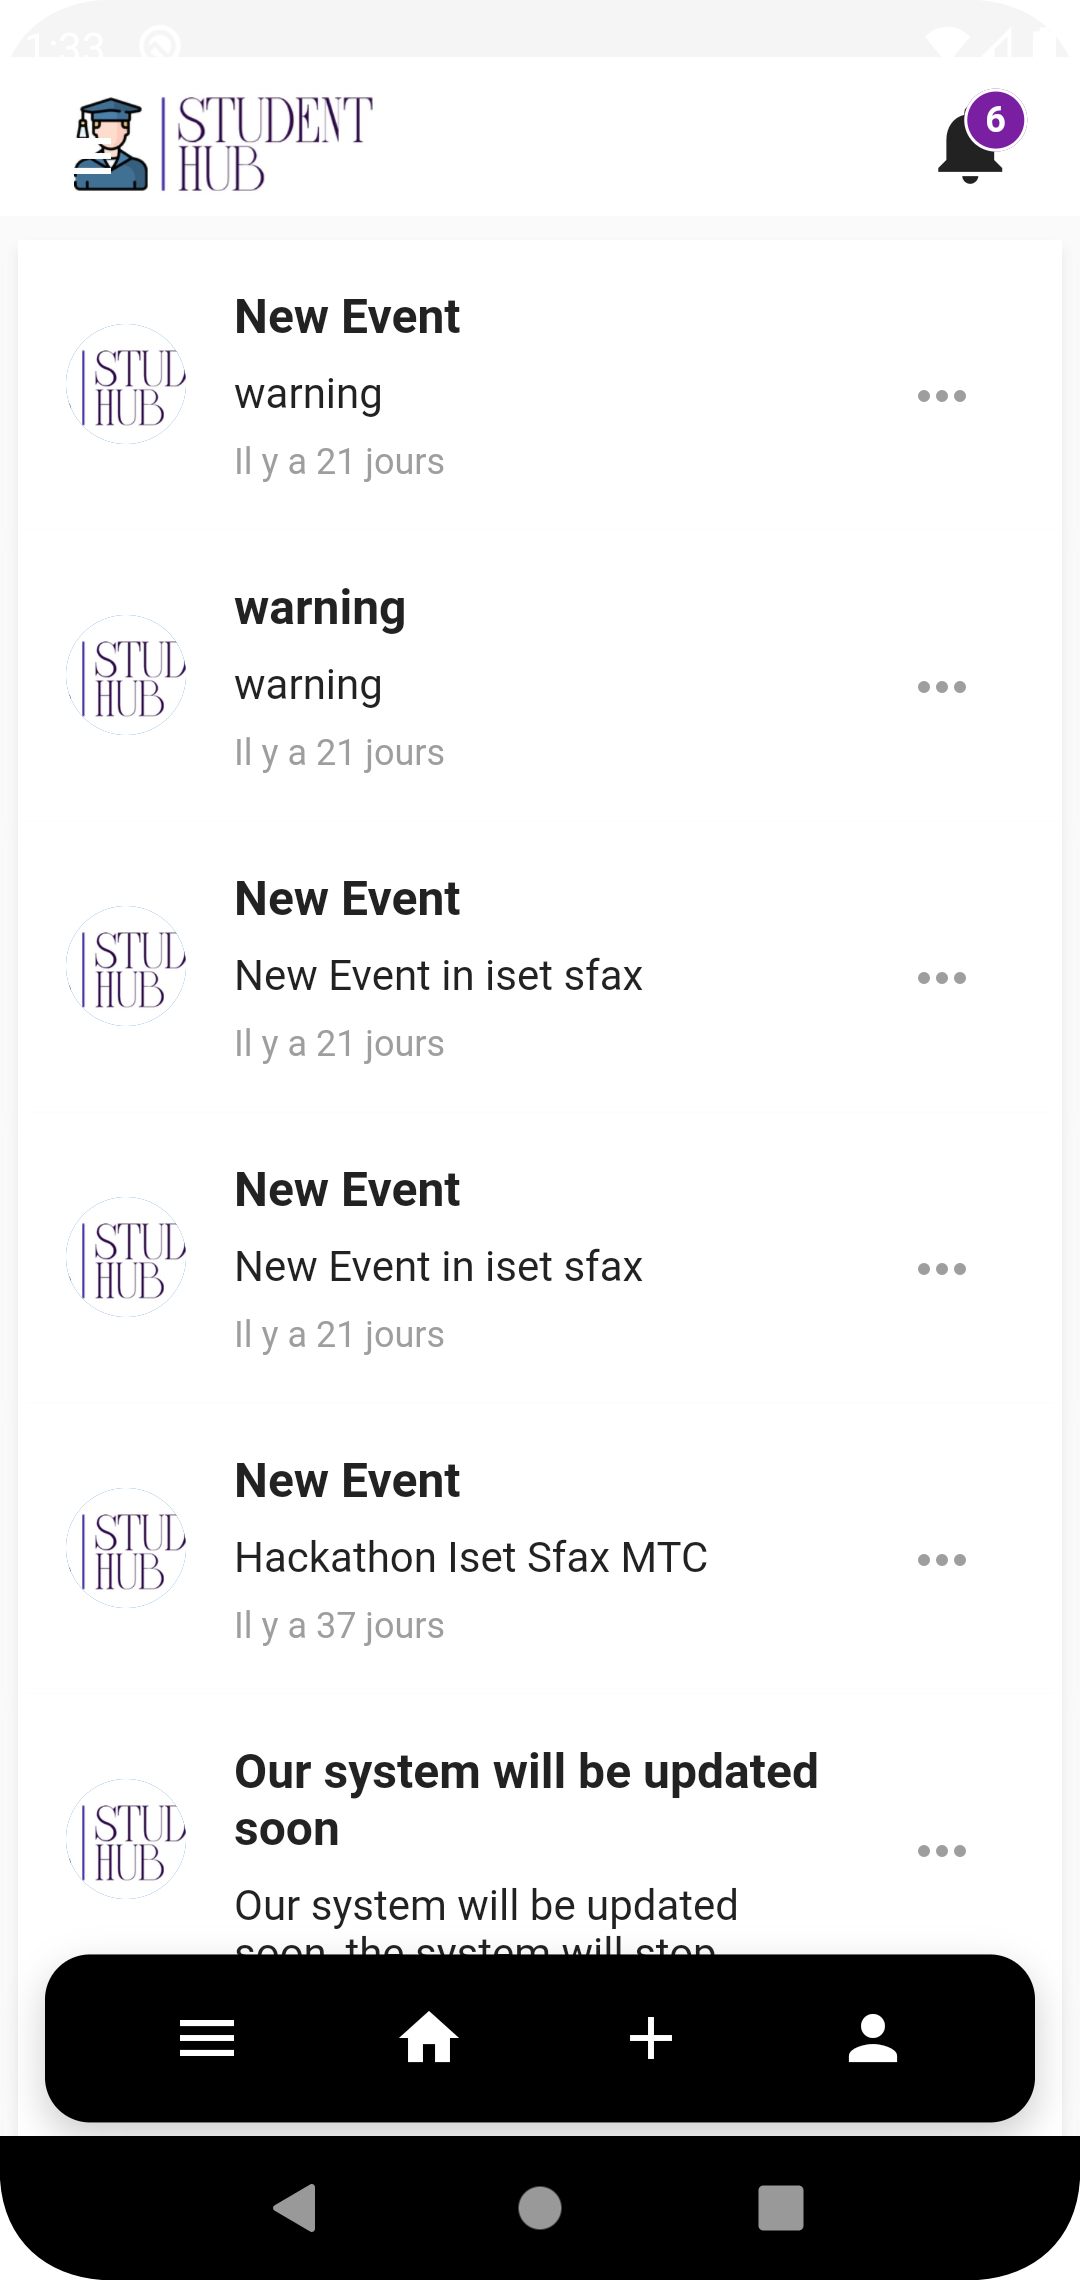
\includegraphics[height=9.5cm,width=7cm]{images/AAANotifications.png}%
    }
    \caption{Interface Notification Partie Mobile}
\end{figure}

\subsection{Interface Notification Personalisée  }
\vspace{-4mm}
L'interface web pour l'administrateur permet de créer des notifications personnalisées. Depuis le tableau de bord, l'administrateur peut accéder à un formulaire pour rédiger le contenu de la notification. Une fois la notification créée et envoyée, elle est visible pour les utilisateurs de l'application mobile, garantissant que les messages importants et spécifiques atteignent rapidement les utilisateurs.

\begin{figure}[H]%
    \center%
    \setlength{\fboxsep}{5pt}%
    \setlength{\fboxrule}{0.5pt}%
    \fbox{
    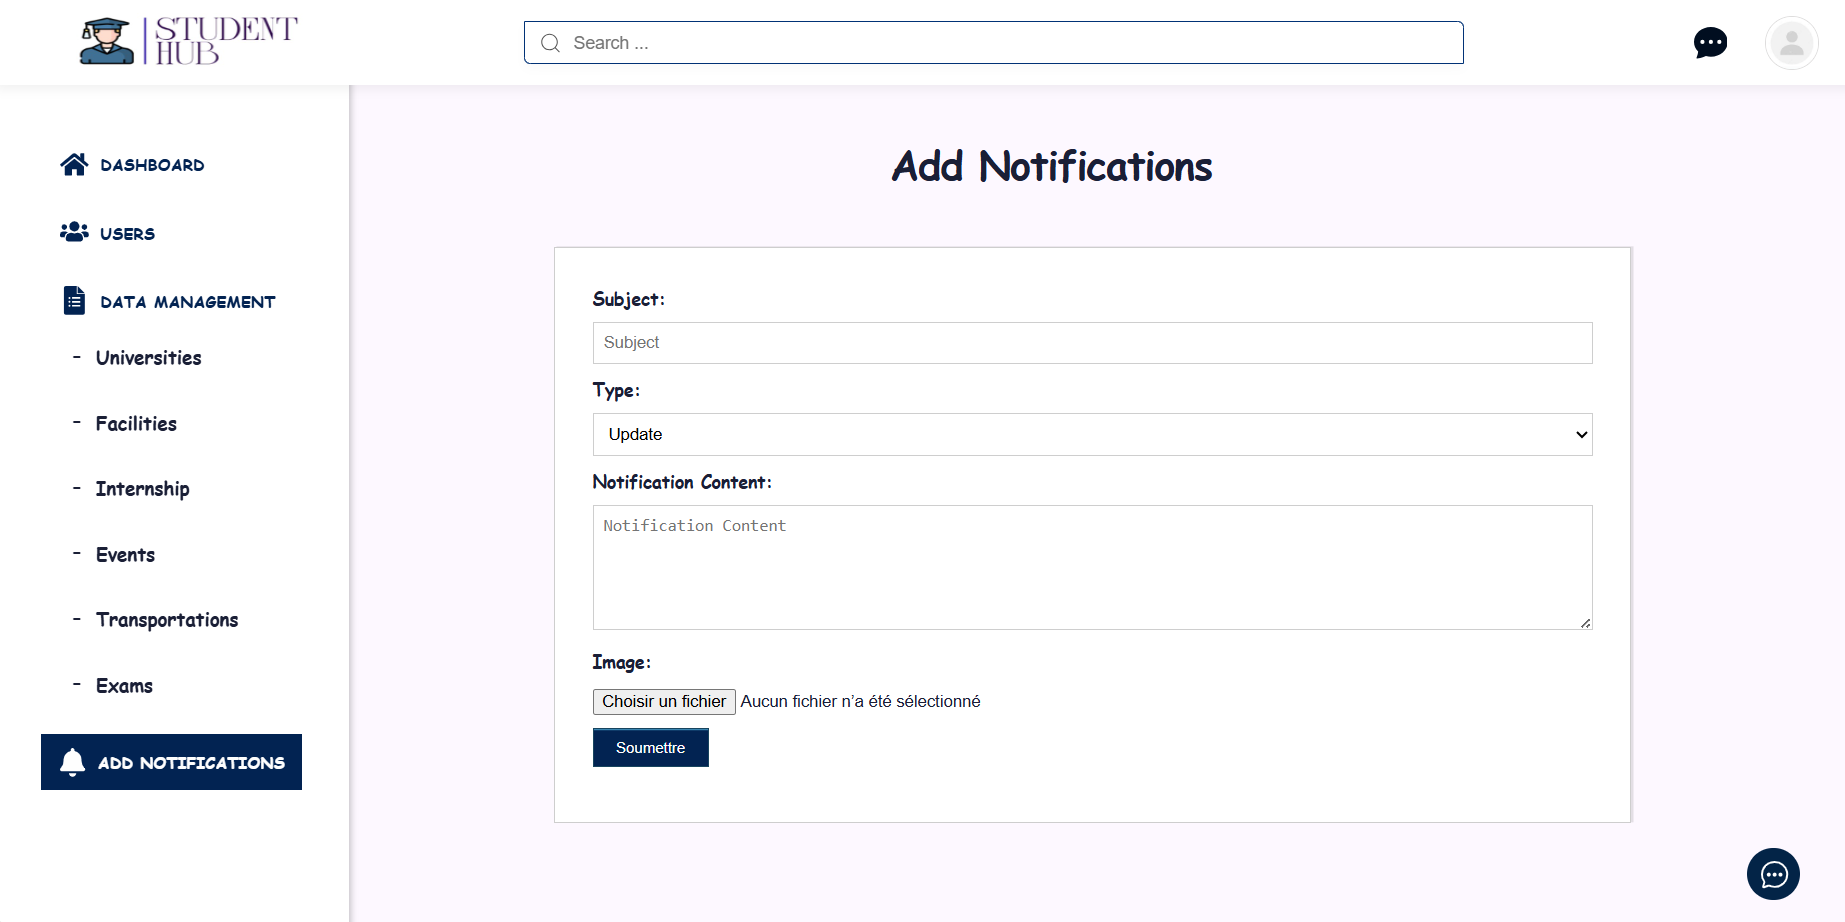
\includegraphics[height=10cm,width=15.5cm]{images/AAAAddNotifications.png}%
    }
    \caption{Interface Notification personalisée }
\end{figure}

\vspace{-1.5cm}
\subsection{Conclusion }
\vspace{-4mm}
En conclusion de ce sprint, nous avons mis en place un système de chat entre l'administration et les étudiants, ainsi qu'un tableau de bord affichant des graphiques pertinents dans la partie web admin. De plus, nous avons introduit une carte interactive pour guider les étudiants et les informer sur leur environnement. Ces ajouts renforcent notre engagement à améliorer l'expérience utilisateur.

\end{sloppypar} 
